La aproximación teórica desarrollada por \parencite{DidiHuberman2011}, en diálogo con las contribuciones fundamentales de \parencite{Benjamin2004} y \parencite{Warburg2010}, establece que el acto de observar una imagen genera significados sobre lo observado. Para los propósitos de esta investigación, resulta fundamental delimitar tanto los elementos teóricos como los instrumentales que guiarán la lectura del corpus de imágenes seleccionado. El campo de los estudios visuales proporciona un marco argumentativo robusto para el análisis de imágenes \parencite{Abril2007}. Este enfoque nos permite construir un escenario metodológico sólido desde el cual aproximarnos, con la necesaria sensibilidad visual, al conjunto de discursos visuales, con el objetivo de elaborar escenarios interpretativos coherentes. Este marco teórico define y proyecta los alcances específicos del trabajo analítico con dichas imágenes.


Como señalan \parencite{Perez2010}:
\begin{quote}
Trabajar con imágenes no sólo es muy entretenido, sino que el proceso de encontrarlas y superponerlas es también muy esclarecedor intelectualmente. Muchas veces primero encuentro la imagen y luego escribo el texto que la acompaña. (p. 45)
\end{quote}

El proceso intelectual de esta investigación comienza con la búsqueda y selección de imágenes. Considerando el extenso impacto mediático del caso de crisis y cierre del Hospital San Juan de Dios (HSJD), se ha realizado una cuidadosa selección que contribuye a la definición de categorías de análisis y codificación.

El caso del San Juan resulta emblemático en el contexto de las crisis sociales e institucionales derivadas de las transformaciones en los sistemas de salud pública, destacándose por su trayectoria histórica como institución hospitalaria fundamental para Bogotá y referente en la medicina suramericana. La complejidad de esta crisis trasciende las explicaciones causales simples, manifestándose como un problema sistémico donde múltiples factores —económicos, políticos, sociales, laborales y simbólicos— se interconectan de manera no-lineal. Esta característica lo sitúa dentro de lo que la teoría de sistemas identifica como problemas de alta complejidad, donde las soluciones tradicionales resultan insuficientes y donde cada intento de intervención puede revelar o crear otros problemas inesperados.

La abundante producción investigativa y comunicativa evidencia su relevancia histórica, legando un importante acervo de información sobre aspectos históricos, sociales, políticos, laborales, médicos y pedagógicos. Sin embargo, esta investigación se centra en las diversas manifestaciones visuales y discursivas como constructoras de sentido, incluyendo tanto las expresiones artísticas como las representaciones institucionales que circulan en torno al HSJD. Dentro de este corpus se encuentran las fotografías de los diferentes eventos protocolarios de reapertura del hospital, reapertura que, como se sabe, nunca se llevó por completo a la realidad. ¿No son acaso las múltiples fotos del evento protocolario de reapertura las que mejor ilustran los anacronismos, supervivencias y la imposibilidad de dar respuesta satisfactoria a las expectativas sobre la reapertura del HSJD? Esta posibilidad será desarrollada más adelante en el capítulo de análisis de las imágenes.

Reconociendo que los enfoques exclusivamente racionales o informativos resultan limitados para capturar la complejidad sistémica del fenómeno, los registros de obra y enunciados visuales se analizan como evidencias que operan mediante lógicas no-verbales, ofreciendo formas de comprensión que complementan y trascienden el conocimiento puramente analítico. Las imágenes artísticas funcionan así como repositorios de una sabiduría práctica que condensa experiencias colectivas y revela aspectos del problema que permanecen ocultos en los análisis puramente informativos. 

Para delimitar el alcance del trabajo con discursos visuales, es importante precisar que no nos limitaremos a un único tipo de imagen. Como señala el iconólogo W.J.T. \parencite{Mitchell2005}, el término ``imagen'' denota tanto el componente físico u objetual como entidades mentales, memoriales y perceptuales. Aunque las imágenes mentales carecen de materialidad física, tienen existencia en nuestro cuerpo y mente, manifestándose a través del lenguaje en el colectivo social.

Las categorías de análisis para las imágenes artísticas relacionadas con la crisis del HSJD incluyen conceptos como: imagen-síntoma, imagen-malicia, imagen-combate, imagen-aura, imagen-fantasma \parencite{DidiHuberman2011}; imagen-virtual, imagen-digital \parencite{Manovich2005}; imagen-dialéctica \parencite{Benjamin2004}; e imagen-tiempo, imagen-movimiento,\linebreak[0] imagen-recuerdo, imagen-sueño \parencite{Deleuze1985}.

\textcolor{edit30sept}{En consecuencia, se adopta la \textit{meta-composición estética y documental} como categoría operativa que hace converger las nociones de \textit{supervivencia}, \textit{anacronismo} y \textit{síntoma} en un dispositivo de montaje. Esta categoría designa la recomposición crítica del archivo visual en escenas que, al tiempo que organizan la mirada, exponen la historicidad discontinua del material y su potencia de sentido no verbal.}

\textcolor{edit30sept}{Este estudio busca enfoques alternativos a la descripción iconológica tradicional, incorporando la búsqueda del anacronismo y el malestar en las imágenes, \textit{el síntoma}. La iconología, según \parencite{Warburg2010}, desobedece la linealidad temporal porque opera mediante supervivencias (\textit{Nachleben}) que permiten que elementos visuales de épocas distantes reaparezcan de manera anacrónica en contextos contemporáneos. Esta desobediencia temporal es fundamental para comprender cómo las imágenes del Hospital San Juan de Dios condensan memorias colectivas que trascienden la cronología factual del cierre hospitalario. La metodología iconológica, al reconocer estas supervivencias, permite identificar cómo gestos, símbolos y patrones visuales migran a través del tiempo, manifestándose como síntomas de latencias sociales que permanecen activas más allá de su contexto histórico original.}

\begin{quote}
    Sería necesario, pues, interrogarse también sobre lo que quiere decir, sobre lo que implica la palabra “síntoma”. Palabra difícil de delimitar: no designa una cosa aislada, ni incluso un proceso reductible a uno o dos vectores, o a un número preciso de componentes. Es una complejidad de segundo grado. No es lo mismo que un concepto semiológico o clínico, incluso cuando compromete una determinada comprensión de la emergencia (fenoménica) del sentido, e incluso si compromete una determinada comprensión de la pregnancia (estructural) de la disfuncionalidad. Esta noción denota por lo menos una doble paradoja, visual y temporal, cuyo interés resulta comprensible para nuestro campo de interrogación sobre las imágenes y el tiempo. \parencite[p. 63]{DidiHuberman2011}
\end{quote}

\begin{figure}[htbp]
    \centering
    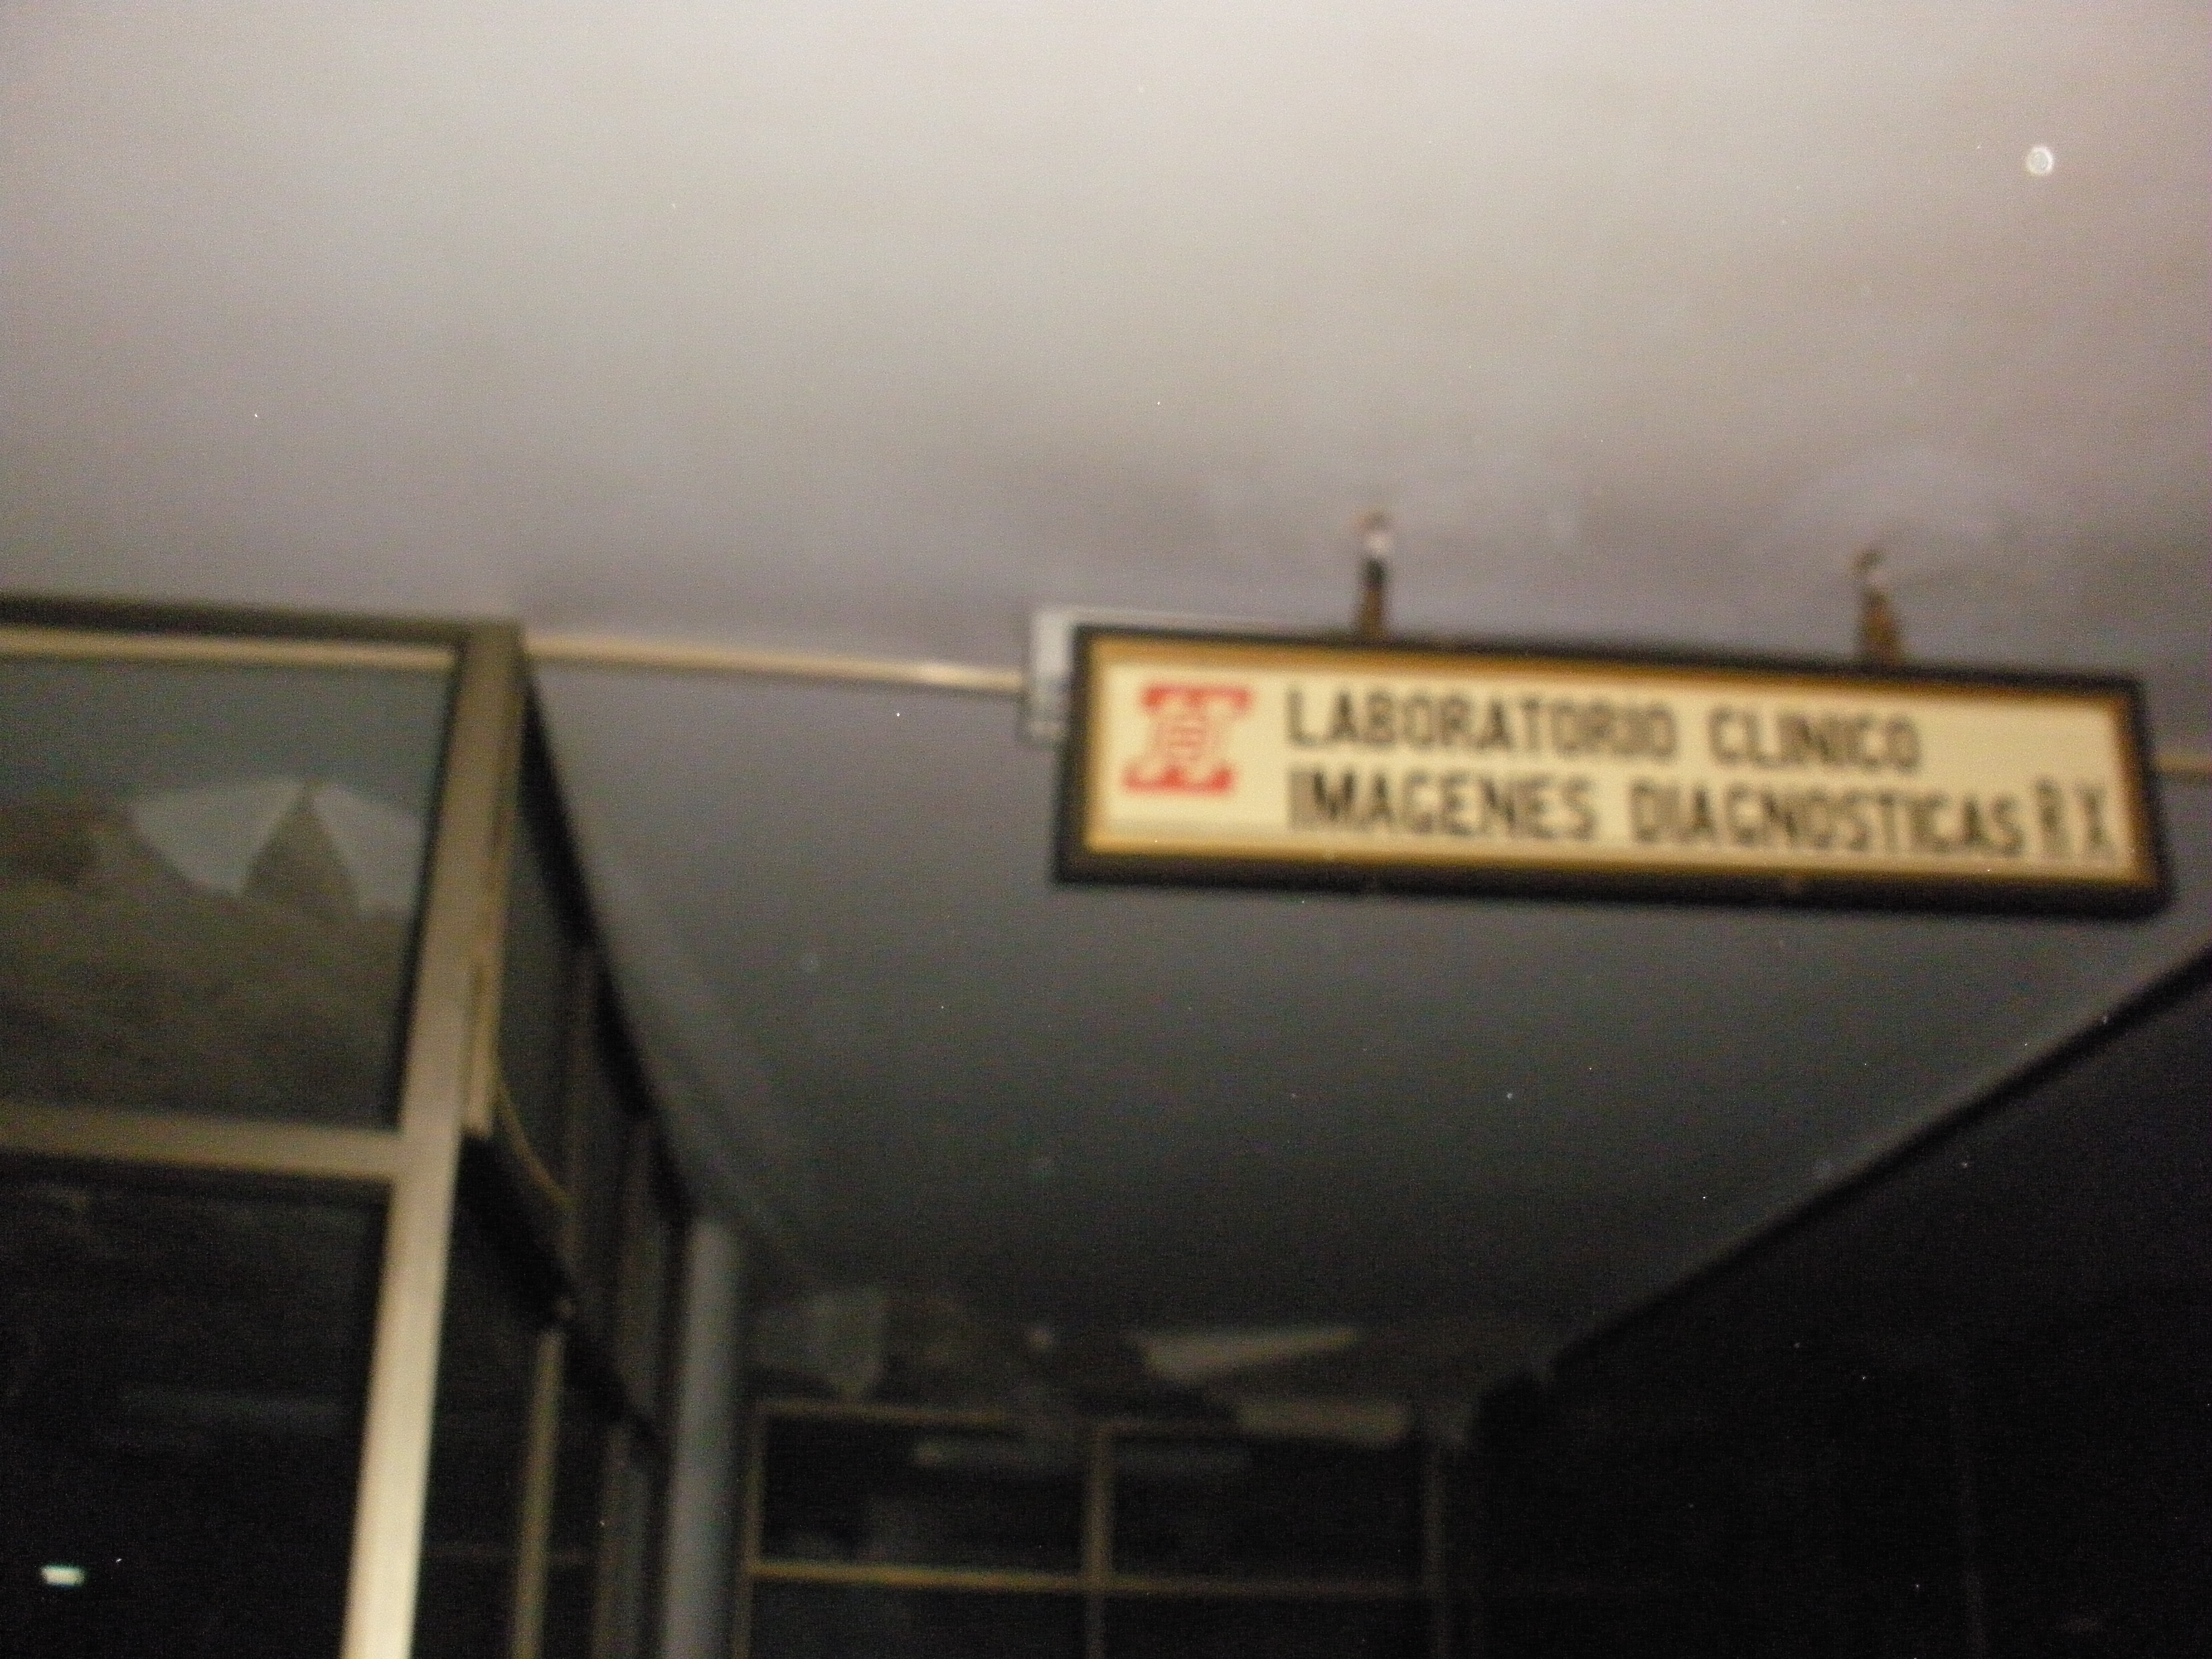
\includegraphics[width=\textwidth]{P7260115.jpg}
    \caption{Señalética imágenes diagnósticas. Foto: Archivo de Margarita Castro.}
    \label{fig:senaletica_imagenes_diagnosticas}
\end{figure}

La investigación se propone profundizar en las relaciones de sentido entre la realidad social y vital del Hospital San Juan de Dios (HSJD) a través del análisis del malestar subyacente en los registros de obra y fotografías testimoniales. Este análisis buscará aplicaciones metodologógicas en dos conceptos teóricos clave: el \textit{montaje}, desarrollado por \parencite{Benjamin2004}, y la noción de \textit{supervivencia} propuesta por \parencite{Warburg2010}. La articulación de estos conceptos permite activar las latencias y síntomas de la memoria social mediante la experiencia visual del observador, operando como una metodología de la sabiduría práctica que trasciende los enfoques puramente informativos o causales. Con esta postura investigativa se adopta el pensamiento a través de imágenes y sus vehículos: los objetos materiales, los medios virtuales y la imaginación, reconociendo que la complejidad sistémica del fenómeno hospitalario demanda formas de conocimiento que integren múltiples temporalidades, perspectivas y modos de comprensión.

\begin{quote}
    Fiction uses imagination as a way of knowing that establishes empathy and intuitively explores the deeper dimensions of events, experiences, and complex human experiences that cannot be fully encapsulated in the literal presentation of facts. \parencite[p. 30]{Leavy2018}
    
    \footnotesize
    (Traducción propia: La ficción utiliza la imaginación como una forma de conocimiento que establece empatía y explora intuitivamente las dimensiones más profundas de los eventos, las experiencias y los complejos aspectos de la condición humana que no pueden ser completamente encapsulados en la presentación literal de los hechos.)
    \normalsize
\end{quote}

Esta perspectiva conecta directamente con la necesidad de enfoques metodológicos que puedan abordar la complejidad sistémica inherente a fenómenos como la crisis del HSJD, donde los análisis exclusivamente racionales o informativos resultan limitados. Las prácticas artísticas, al igual que la ficción, operan mediante lógicas no-lineales que pueden capturar aspectos de la experiencia colectiva que permanecen inaccesibles para enfoques puramente documentales. En este sentido, las imágenes artísticas funcionan como condensadores de sabiduría práctica, integrando dimensiones emocionales, simbólicas y experienciales que complementan el conocimiento puramente factual.

\section{Imagen-síntoma}

El análisis de las imágenes artísticas, registros de obra y fotografías testimoniales relacionadas con el Hospital San Juan de Dios (HSJD) requiere establecer un marco de referencia específico. Este marco busca construir un escenario que permita al observador organizar visualmente los atributos de las imágenes, facilitando la incorporación de valores de sentido no-textuales sobre este fenómeno sociocultural.

En el conjunto de manifestaciones artísticas y visuales vinculadas al HSJD, se evidencian emergencias visuales que operan como metáforas de patologías sociales, materializando los síntomas de un momento de crisis. Para analizar estas relaciones y el valor de sentido en la imagen, resulta fundamental establecer las conexiones entre la construcción de sentido y la imagen, lo que denominamos imagen-síntoma. Esta manifestación sintética no se limita al ámbito de la producción artística formal, sino que se extiende a las expresiones espontáneas de la ciudadanía que, frente a las narrativas oficiales sobre el hospital, generan respuestas que revelan malestares profundos en la representación social del fenómeno. Las conversaciones públicas en medios digitales evidencian este carácter sintético cuando expresan: ``esto es ridículo se necesita una reforma de justicia''\footnote{Facebook. Comentarios en publicación 108379099286148\_453423351448386. Fecha de consulta: [2015]. Corpus de conversaciones digitales sobre HSJD.} o ``es un insulto atribuirle ese mérito [...] y muy ofensivo que pretendan engañar a los ciudadanos''\footnote{Facebook. Comentarios en publicación 108379099286148\_453423351448386. Fecha de consulta: [2015]. Corpus de conversaciones digitales sobre HSJD.}. La dimensión sintomática se intensifica cuando la ciudadanía denuncia explícitamente la manipulación simbólica: ``Eso no es San Juan de Dios, es un centro de consulta prioritaria en las instalaciones de lo que fué la casa de la escuela de Medicina de la Universidad Nacional y el Hospital más antiguo de Suramérica. IMBÉCILES los de la 'administración' distrital llenándose la boca diciendo que abrieron San Juan, tratando de engañarnos a todos''\footnote{Facebook. Comentarios en publicación 108379099286148\_453423351448386. Usuario: Aldo Beltrán. Fecha de consulta: [2015]. Corpus de conversaciones digitales sobre HSJD.}. Estas manifestaciones no constituyen simplemente opiniones, sino emergencias visuales que operan como síntomas de una crisis de representación más profunda, donde la disputa por el sentido del hospital trasciende la mera discusión política para convertirse en una lucha por la legitimidad de las narrativas sobre la memoria colectiva.

\textcolor{edit30sept}{La imagen-síntoma, de acuerdo con \parencite{DidiHuberman2011}, articula dos fuerzas complementarias: la reiteración de elementos visuales preexistentes y la alteridad que estos adquieren al emerger fuera de sus contextos habituales. En el análisis de las representaciones del HSJD, esta categoría permite captar aquellas manifestaciones visuales que, al conservar huellas de una memoria colectiva latente, desestabilizan las lecturas convencionales y revelan tensiones en la narrativa oficial.} Este concepto abarca las supervivencias, latencias y reapariciones que habitan en las imágenes, elementos que \parencite{Warburg2010} identifica como formas persistentes de la memoria visual colectiva. En el caso del HSJD, estas supervivencias se manifiestan no solo en las obras artísticas formales, sino también en la persistencia de una imagen idealizada del hospital como ``el mejor hospital público'' que se mantiene activa en la memoria ciudadana, operando como un fantasma que sobrevive a la realidad física del edificio cerrado. Esta supervivencia simbóblica genera una tensión permanente entre lo que el hospital fue, lo que representa en la memoria colectiva y lo que se pretende que sea en las narrativas contemporáneas. La imagen-síntoma surge precisamente de esta tensión, revelando las fisuras en la representación oficial y activando memorias que resistían ser incorporadas en los discursos hegemónicos sobre la transformación urbana y las políticas de salud.

\begin{quote}
¿Qué es, en efecto, un síntoma si no el signo inadvertido, no familiar, a menudo intenso y siempre disruptivo, que anuncia visualmente algo que no es todavía visible, algo que todavía no conocemos? Si la imagen es un síntoma -en el sentido crítico y no clínico del término-, si la imagen es un malestar en la representación, es porque indica un futuro de la representación, un futuro que no sabemos aún leer, ni, incluso, describir. \parencite[p. 307]{DidiHuberman2011}
\end{quote}

\subsection*{Sentido crítico y no clínico del síntoma}

La noción de síntoma en la crítica visual y cultural trasciende su acepción médica tradicional. \parencite{DidiHuberman2011} desarrolla este concepto como una manifestación que irrumpe en el curso \textcolor{edit30sept}{normativizado} de la representación, revelando dimensiones latentes e inconscientes tanto de la historia como de la imagen misma. Estas manifestaciones, lejos de ser simples anomalías, poseen un carácter crítico y disruptivo que cuestiona las certezas establecidas y las cronologías tradicionales. En el contexto del HSJD, el sentido crítico del síntoma se manifiesta en la capacidad de las imágenes artísticas para revelar aspectos del problema hospitalario que permanecen invisibles en los análisis puramente informativos o administrativos. El síntoma visual opera entonces como una forma de conocimiento que no se limita a diagnosticar estados presentes, sino que revela potencialidades latentes y futuros posibles que aún no han encontrado articulación discursiva.

La genealogía conceptual del síntoma visual encuentra sus raíces en el psicoanálisis freudiano, particularmente en los estudios sobre procesos de condensación y desplazamiento. \parencite{DidiHuberman2011} expande este marco analítico al campo visual, sugiriendo que las imágenes operan de manera análoga al ``trabajo del sueño'', condensando significados múltiples y revelando aspectos no visibles o no reconocidos. Esta operación no se limita al ámbito de las imágenes artísticas formales, sino que se extiende a todas las formas de producción visual que emergen en torno al fenómeno hospitalario, incluyendo las manifestaciones espontáneas en espacios digitales donde la ciudadanía elabora sus propias ``imágenes'' discursivas del problema. La condensación opera cuando múltiples temporalidades se superponen en una sola expresión: ``el alcalde que lo cerró hace 15 años'' condensa tanto la memoria de la clausura como la crítica al presente, mientras que el desplazamiento se evidencia cuando la frustración por las políticas de salud se desplaza hacia el debate sobre la autoría de los proyectos de reapertura.

Como señala \parencite[p. 37]{VegaArevalo2017}:

\begin{quote}
    La idea de la imagen como síntoma es lo que quiere tomar Didi-Huberman de Freud y aplicarlo al campo de la historia del arte. Por supuesto, no sobra decir que se trata de dos disciplinas muy distintas, que la experiencia de las imágenes oníricas no es igual a la de las imágenes artísticas. Aun así, el uso del carácter sintomático de la imagen en la historia del arte no es tan diferente al del análisis de los sueños. Sólo que aquí, en lugar de evocar lo onírico, Didi-Huberman lo utilizará para nombrar esa perturbación que lo visual causa dentro de lo visible: ``en un cuadro de pintura figurativa <<algo representa>> y <<algo se ve>> -pero algo [...] se muestra también, se mira, nos mira-''
\end{quote}

El concepto de \textit{Denkbild}, desarrollado por \parencite{Benjamin2004}, constituye una herramienta analítica complementaria para identificar estos síntomas visuales en el ámbito del pensamiento crítico. Estos síntomas representan manifestaciones simbólicas de tensiones culturales, sociales e históricas que trascienden su apariencia inmediata. A través del \textit{Denkbild}, Benjamin demuestra cómo ciertos objetos, escenas o fragmentos de la cotidianidad encapsulan dinámicas profundas esenciales para una crítica reflexiva.

Esta perspectiva conecta directamente con la noción benjaminiana del narrador como figura portadora de sabiduría práctica, quien ``tiene consejo no para unas pocas situaciones, como el proverbio, sino para muchas, como el sabio''. Las imágenes artísticas sobre el HSJD operan de manera análoga: condensan experiencias colectivas y ofrecen formas de comprensión que no se limitan a la información factual sino que integran dimensiones temporales complejas, memorias latentes y supervivencias simbólicas. Esta sabiduría visual se caracteriza por su capacidad de articular conocimientos que emergen de la experiencia vivida y que resisten la reducción a explicaciones causales simples. En contraste con la información que, según Benjamin, ``no sobrevive al momento en que fue nueva'', las imágenes-síntoma del hospital conservan su potencia reveladora a través del tiempo, activando comprensiones que permanecían inaccesibles para los enfoques puramente informativos o documentales.

Esta capacidad de supervivencia de la sabiduría visual se manifiesta concretamente en la persistencia de imágenes idealizadas del hospital que trascienden su realidad física inmediata. La referencia ciudadana al HSJD como ``baluarte que ahora es de la ciudad''\footnote{X (antes Twitter). Cuenta: https://x.com/AmigosdelSJ. Fecha de consulta: [2015]. Corpus de conversaciones digitales sobre HSJD.} revela cómo ciertas imágenes conservan su potencia simbólica independientemente de las transformaciones materiales del edificio. Esta supervivencia se profundiza cuando la memoria colectiva preserva la dimensión formativa del hospital: ``Da mucha alegría saber que este hospital donde se formaron y nos formamos muchos profesionales de la salud de nuevo vuelve a ser de la comunidad y para la comunidad''\footnote{Facebook. Comentarios en publicación 108379099286148\_453423351448386. Usuario: Marcela Cordoba. Fecha de consulta: [2015]. Corpus de conversaciones digitales sobre HSJD.}, evidenciando cómo la institución trasciende su función asistencial para constituirse como espacio de transmisión generacional del conocimiento médico. La dimensión patrimonial de esta supervivencia se manifiesta cuando la ciudadanía evoca al hospital como ``templo de la medicina'': ``así como se hizo teletón se debería hacer una cruzada nacional para recaudar y abrir el san juan quien no pasó por allí como estudiante o como paciente es un templo de la medicina''\footnote{Facebook. Comentarios en publicación 108379099286148\_453423351448386. Usuario: Harold Fabricio Hernandez Cruz. Fecha de consulta: [2015]. Corpus de conversaciones digitales sobre HSJD.}. Esta persistencia no constituye una simple nostalgia, sino una forma activa de sabiduría práctica que mantiene viva la posibilidad de futuros alternativos para la institución hospitalaria. Las imágenes artísticas y las manifestaciones ciudadanas espontaneas funcionan entonces como repositorios de esta sabiduría, conservando y transmitiendo conocimientos sobre el cuidado, la resistencia y la supervivencia institucional que no pueden ser completamente articulados a través de los discursos puramente racionales o administrativos.

\section{Anacronismo}

El anacronismo, entendido como la intrusión de una época en otra, constituye un concepto fundamental en la antropología de las imágenes desarrollada por \parencite{DidiHuberman2011}. Este enfoque nos permite abordar la compleja temporalidad inherente a las imágenes, exponiéndolas a interpretaciones insospechadas y lógicas no convencionales. La identificación y análisis de estos anacronismos se convierte en una herramienta metodológica esencial para develar el sentido a través de las huellas de la memoria social manifiestas en la imagen artística. En el contexto del HSJD, el anacronismo opera de manera particularmente reveladora, pues las conversaciones públicas sobre el hospital evidencian cómo múltiples temporalidades se superponen y chocan en un mismo espacio discursivo: ``el alcalde que lo cerró hace 15 años''\footnote{X (antes Twitter). Cuenta: https://x.com/AmigosdelSJ. Fecha de consulta: [2015]. Corpus de conversaciones digitales sobre HSJD.}, ``la administración anterior''\footnote{Facebook. Comentarios en publicación 108379099286148\_453423351448386. Fecha de consulta: [2015]. Corpus de conversaciones digitales sobre HSJD.}, ``desde enero de 2016''\footnote{X (antes Twitter). Cuenta: https://x.com/AmigosdelSJ. Fecha de consulta: [2015]. Corpus de conversaciones digitales sobre HSJD.}, ``lo que fue antes el San juan, el mejor hospital público''\footnote{Facebook. Comentarios en publicación 108379099286148\_453423351448386. Fecha de consulta: [2015]. Corpus de conversaciones digitales sobre HSJD.}. Estas referencias no constituyen simplemente marcadores cronológicos, sino constelaciones anacrónicas donde el pasado irrumpe en el presente, el presente se proyecta hacia el pasado, y las imágenes idealizadas del hospital coexisten con las realidades contemporáneas de manera no-lineal. La complejidad anacrónica se evidencia cuando estudiantes actuales reclaman continuidad institucional: ``Soy estudiante de medicina de la Universidad Nacional y me gustaría saber que paso con el papel que teníamos en mencionada institución, y cuál sera nuestro papel ahora, puesto que si ese hospital es emblemático, es por el aporte inmenso de la Nacional a la salud en el país''\footnote{Facebook. Comentarios en publicación 108379099286148\_453423351448386. Usuario: Alvaro Daniel Patiño. Fecha de consulta: [2015]. Corpus de conversaciones digitales sobre HSJD.}. El anacronismo revela así cómo la memoria del hospital funciona mediante superposiciones temporales que resisten la organización secuencial de la historia oficial.

Como señala Didi-Huberman: 

\begin{quote}
    El anacronismo parece surgir en el pliegue exacto de la relación entre imagen e historia; las imágenes, desde luego, tienen una historia; pero lo que ellas son, su movimiento propio, su poder específico, no aparece en la historia más que como un síntoma -un malestar, una desmentida más o menos violenta, una suspensión'' \parencite[p. 48]{DidiHuberman2011}.
\end{quote}

Al situarnos ante una imagen, nos encontramos simultáneamente ante un tiempo no cronológico. La temporalidad en la imagen reside en nuestra imaginación y trasciende la secuencialidad convencional. La dimensión memorativa de la imagen se proyecta en el inconsciente y se manifiesta a través de superposiciones temporales, revelando así atributos fundamentales de la memoria social. En el caso específico del HSJD, estas superposiciones temporales adquieren una densidad particular, pues las imágenes del hospital condensan no solo la historia de una institución específica, sino también la historia de las transformaciones urbanas de Bogotá, los cambios en las políticas de salud pública, las luchas sociales por el derecho a la salud, y las supervivencias de modelos hospitalarios alternativos al modelo neoliberal. Esta condensación temporal no opera mediante causalidades lineales, sino a través de resonancias, ecos y retornos que activan memorias latentes en el observador. Las imágenes artísticas del hospital funcionan entonces como catalizadores de estos procesos anacrónicos, liberando temporalidades que habían sido reprimidas o marginalizadas en las narrativas hegemónicas sobre el desarrollo urbano y las políticas sanitarias.

El choque de temporalidades en la imagen libera todas las modalidades del tiempo mismo, elaborando una paradoja: mientras la imagen en la historia se dispersa, también se cristaliza en obras concretas. Las imágenes contienen frágiles supervivencias que nos conmueven y permiten una comprensión no verbal de los fenómenos complejos. Esta capacidad de las imágenes para articular temporalidades múltiples las convierte en herramientas privilegiadas para abordar problemas de alta complejidad sistémica, donde las relaciones causales lineales resultan insuficientes. Las imágenes anacrónicas del HSJD no solo documentan un momento histórico específico, sino que activan constelaciones de sentido que conectan crisis hospitalarias, transformaciones urbanas, resistencias sociales y supervivencias simbólicas en configuraciones que trascienden cronologías simples.

\textcolor{edit30sept}{Por lo tanto, al desmontar el registro de obra plástica, documental, fotográfica, dramatúrgica o performática de su función y contexto de producción original, podemos revelar aspectos del fenómeno que trascienden los motivos iconológicos evidentes. Este desmontaje opera como un condensador de experiencias colectivas que resisten la reducción a explicaciones unidimensionales. La iconología desobedece la linealidad porque reconoce que las imágenes operan mediante la lógica del montaje, concepto desarrollado por \cite{Benjamin2004}, donde elementos heterogéneos y temporalmente distantes se articulan produciendo nuevos significados críticos. Las imágenes se convierten así en vehículos de un conocimiento contextual y relacional que complementa y enriquece los análisis puramente racionales, ofreciendo perspectivas múltiples sobre un problema cuya complejidad sistémica demanda enfoques igualmente complejos y multidimensionales. Esta aproximación iconológica revela cómo las manifestaciones visuales del HSJD condensan simultaneidades temporales que escapan a la narración histórica lineal, activando memorias y potencialidades que operan como síntomas de expresiones discursicas no articuladas.}

Esta metodología del desmontaje encuentra su fundamento teórico en el concepto benjaminiano de \textit{montaje}, que opera no mediante síntesis dialécticas tradicionales, sino a través de la construcción de constelaciones donde los elementos yuxtapuestos generan ``chispas'' de comprensión. En el corpus visual del HSJD, estas constelaciones se manifiestan cuando diferentes registros —desde el programa ``Madre Canguro'' que ``fue pionero en el mundo''\footnote{X (antes Twitter). Cuenta: https://x.com/AmigosdelSJ. Tweet del 2 de febrero de 2015. Corpus de conversaciones digitales sobre HSJD.} hasta ``la huerta que se utilizaba para hacer terapias a las personas con patologías''\footnote{X (antes Twitter). Cuenta: https://x.com/AmigosdelSJ. Tweet del 22 de febrero de 2015. Corpus de conversaciones digitales sobre HSJD.}, pasando por el ``jardín infantil del San Juan de Dios'' que ``será reabierto''\footnote{X (antes Twitter). Cuenta: https://x.com/AmigosdelSJ. Tweet del 21 de febrero de 2015. Corpus de conversaciones digitales sobre HSJD.} y la memoria de que ``en este hospital se formaron los maestros de los demás médicos de nuestro país''\footnote{X (antes Twitter). Cuenta: https://x.com/AmigosdelSJ. Tweet del 11 de febrero de 2015. Corpus de conversaciones digitales sobre HSJD.}— se articulan no de manera secuencial sino anacrónica, creando un montaje del hospital como espacio integral de cuidado que trasciende las limitaciones de su realidad física inmediata. Este montaje anacrónico revela cómo la resistencia y supervivencia simbólica del hospital no dependen únicamente de su reapertura física, sino de la capacidad de las imágenes para mantener activas las potencialidades latentes de modelos alternativos de atención sanitaria y cuidado comunitario. La metodología visual propuesta permite así acceder a dimensiones del fenómeno hospitalario que permanecen inaccesibles para los enfoques puramente administrativos, políticos o médicos, revelando la persistencia de sabidurías prácticas sobre el cuidado que resisten su instrumentalización o mercantilización.

